\section{Atividades}

\subsection{Atividade 1 -- Preparação do Ambiente}

\paragraph{}
Inicialmente foi realizada a validação do ambiente de laboratório, garantindo
que as máquinas \texttt{atacante} e \texttt{alvo} estavam em execução e
acessíveis para os testes propostos.

\paragraph{}
Em seguida foi utilizada a ferramenta \texttt{curl} para verificar a
disponibilidade da API hospedada em \texttt{api.vulneravel.com}.

\paragraph{}
A resposta obtida confirmou o funcionamento correto do serviço e demonstrou que
a API estava pronta para ser analisada durante as etapas seguintes da atividade.

\subsection{Atividade 2 -- Varredura de Informações da API}

\paragraph{}
Foi realizada uma etapa de reconhecimento da API utilizando a documentação
Swagger disponibilizada pelo sistema.

\paragraph{}
A análise permitiu identificar os endpoints disponíveis, os métodos HTTP
aceitos e os recursos que poderiam ser acessados por usuários autenticados ou
não autenticados.

\paragraph{}
Utilizando a ferramenta \texttt{curl}, foram realizadas consultas em diferentes
rotas da API com o objetivo de identificar informações expostas
indevidamente.

\paragraph{}
Durante essa análise foi identificado um endpoint de depuração que retornava
informações sensíveis dos usuários cadastrados, incluindo senhas e privilégios
administrativos, caracterizando uma vulnerabilidade de exposição excessiva de
dados.

\begin{figure}[H]
\centering
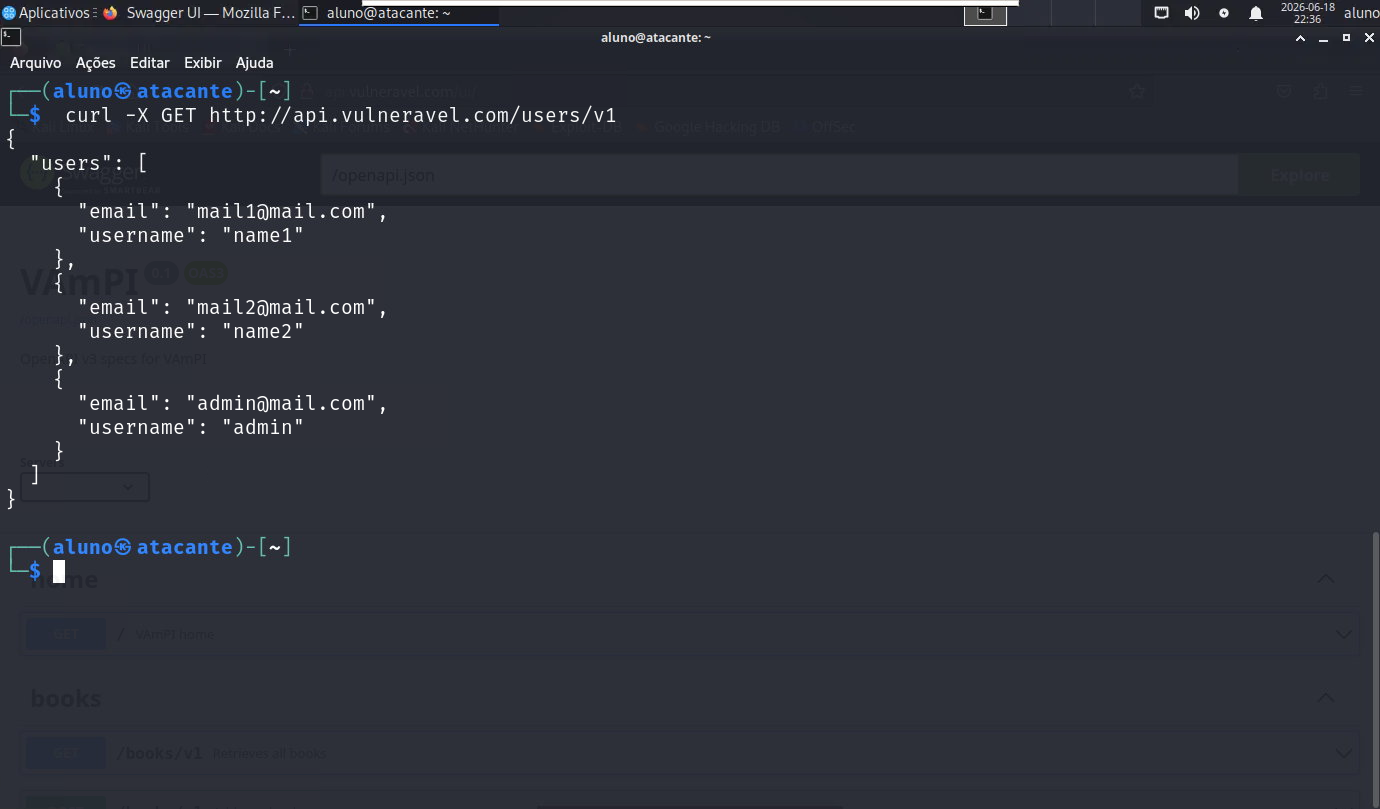
\includegraphics[width=0.95\textwidth]{./fig/varredura-api.png}
\caption{Varredura e enumeração de informações da API utilizando curl.}
\end{figure}

\paragraph{}
Também foi realizado o cadastro de um novo usuário e a obtenção de um token de
autenticação válido para utilização nas atividades posteriores.

\paragraph{}
Além disso, foi explorada uma vulnerabilidade do tipo BOLA/IDOR, permitindo o
acesso a informações privadas associadas a recursos pertencentes a outros
usuários apenas modificando identificadores presentes na URL.

\subsection{Atividade 3 -- Exploração de SQL Injection}

\paragraph{}
Foi realizada uma análise do endpoint responsável pela consulta de usuários,
buscando identificar possíveis falhas de validação de entrada.

\paragraph{}
Durante os testes observou-se que a aplicação aceitava caracteres especiais na
URL sem realizar o tratamento adequado das entradas fornecidas pelo usuário.

\paragraph{}
Após a confirmação do comportamento suspeito, foi utilizada a ferramenta
\texttt{SQLMap} para automatizar a identificação dos pontos vulneráveis.

\paragraph{}
A ferramenta confirmou a existência de vulnerabilidades de SQL Injection,
permitindo a execução de consultas manipuladas e demonstrando a possibilidade
de acesso indevido às informações armazenadas no banco de dados.

\begin{figure}[H]
\centering
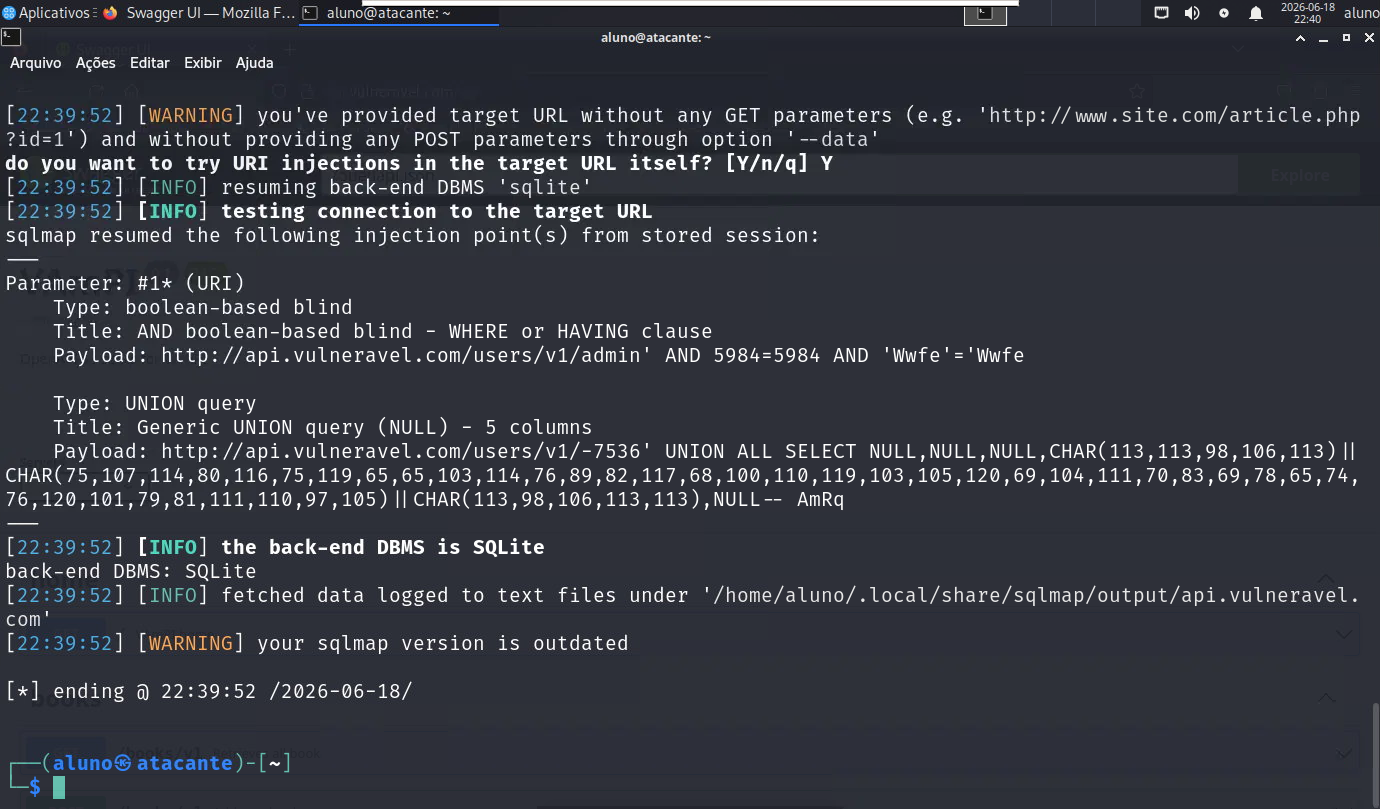
\includegraphics[width=0.95\textwidth]{./fig/sql-injection.png}
\caption{Identificação da vulnerabilidade de SQL Injection utilizando SQLMap.}
\end{figure}

\subsection{Atividade 4 -- Exploração de Mass Assignment}

\paragraph{}
Foi analisado o processo de cadastro de novos usuários disponibilizado pela
API.

\paragraph{}
Durante os testes verificou-se que o sistema aceitava parâmetros adicionais não
documentados na requisição de registro.

\paragraph{}
Explorando esse comportamento, foi possível adicionar manualmente o atributo
\texttt{admin=true} durante a criação de uma nova conta.

\paragraph{}
O sistema processou a requisição sem qualquer validação adicional, resultando
na criação de um usuário com privilégios administrativos.

\paragraph{}
A vulnerabilidade identificada caracteriza um caso de \textit{Mass Assignment},
onde atributos internos da aplicação podem ser manipulados diretamente por um
usuário não autorizado.

\begin{figure}[H]
\centering
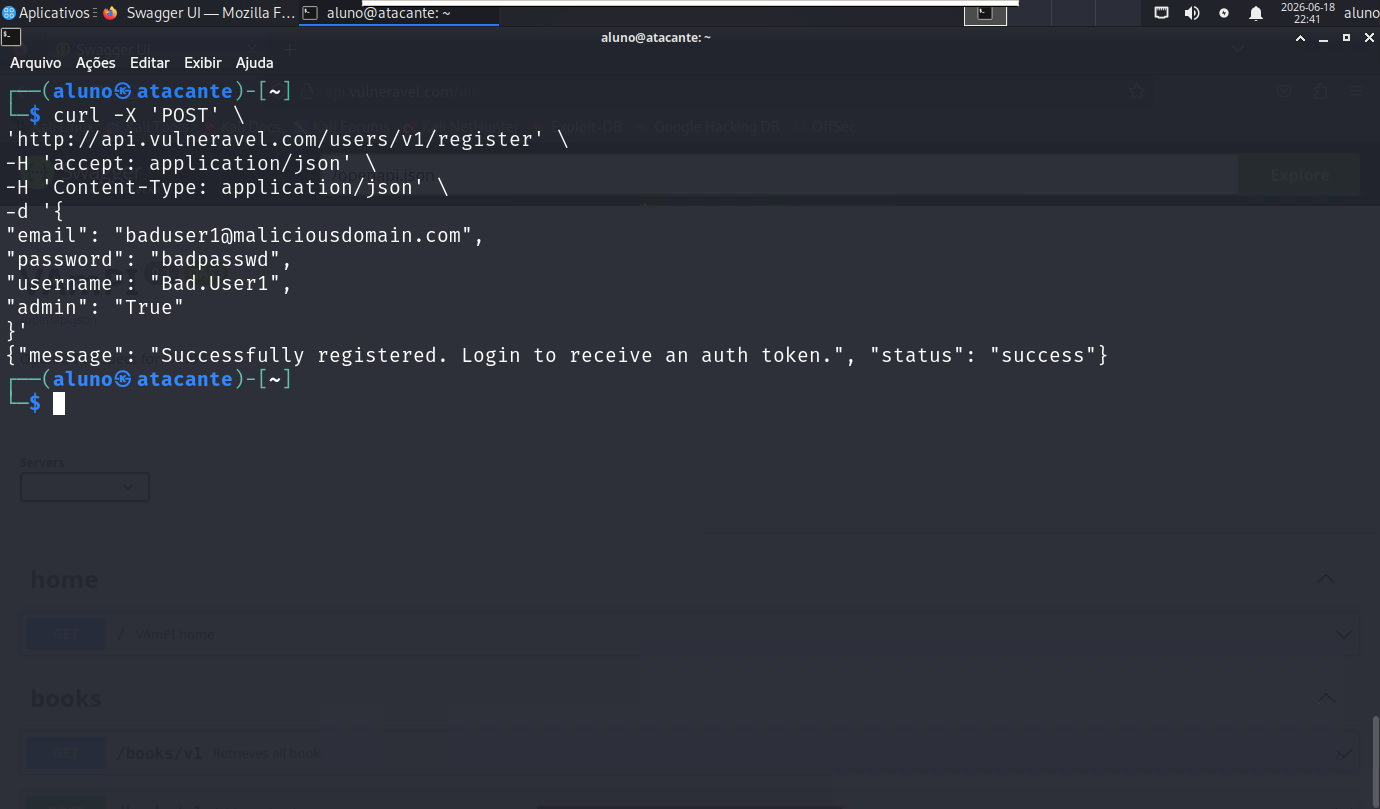
\includegraphics[width=0.95\textwidth]{./fig/mass-assignment.png}
\caption{Criação de usuário administrativo através da vulnerabilidade Mass Assignment.}
\end{figure}

\subsection{Atividade 5 -- Exploração de Unauthorized Password Change}

\paragraph{}
Foi realizado o processo de autenticação utilizando uma conta comum do sistema,
obtendo um token de acesso válido.

\paragraph{}
Em seguida foram analisadas as funcionalidades disponíveis para atualização de
dados dos usuários.

\paragraph{}
Durante os testes verificou-se que o endpoint responsável pela alteração de
senhas não validava adequadamente a autorização do usuário autenticado.

\paragraph{}
Explorando essa falha, foi possível alterar a senha da conta administrativa
utilizando apenas as credenciais de um usuário comum. Durante o teste, foi
realizada autenticação com o usuário \texttt{name1} e, mesmo sem privilégios
administrativos, a aplicação permitiu a alteração da senha da conta
\texttt{admin}, modificando seu valor para \texttt{HACKED}.

\paragraph{}
Após a execução do ataque, uma nova consulta aos dados internos da API
confirmou que a senha do administrador havia sido modificada com sucesso.

\paragraph{}
Essa vulnerabilidade demonstra uma falha crítica de controle de acesso, pois
permite que usuários sem privilégios realizem alterações em contas de
terceiros.

\begin{figure}[H]
\centering
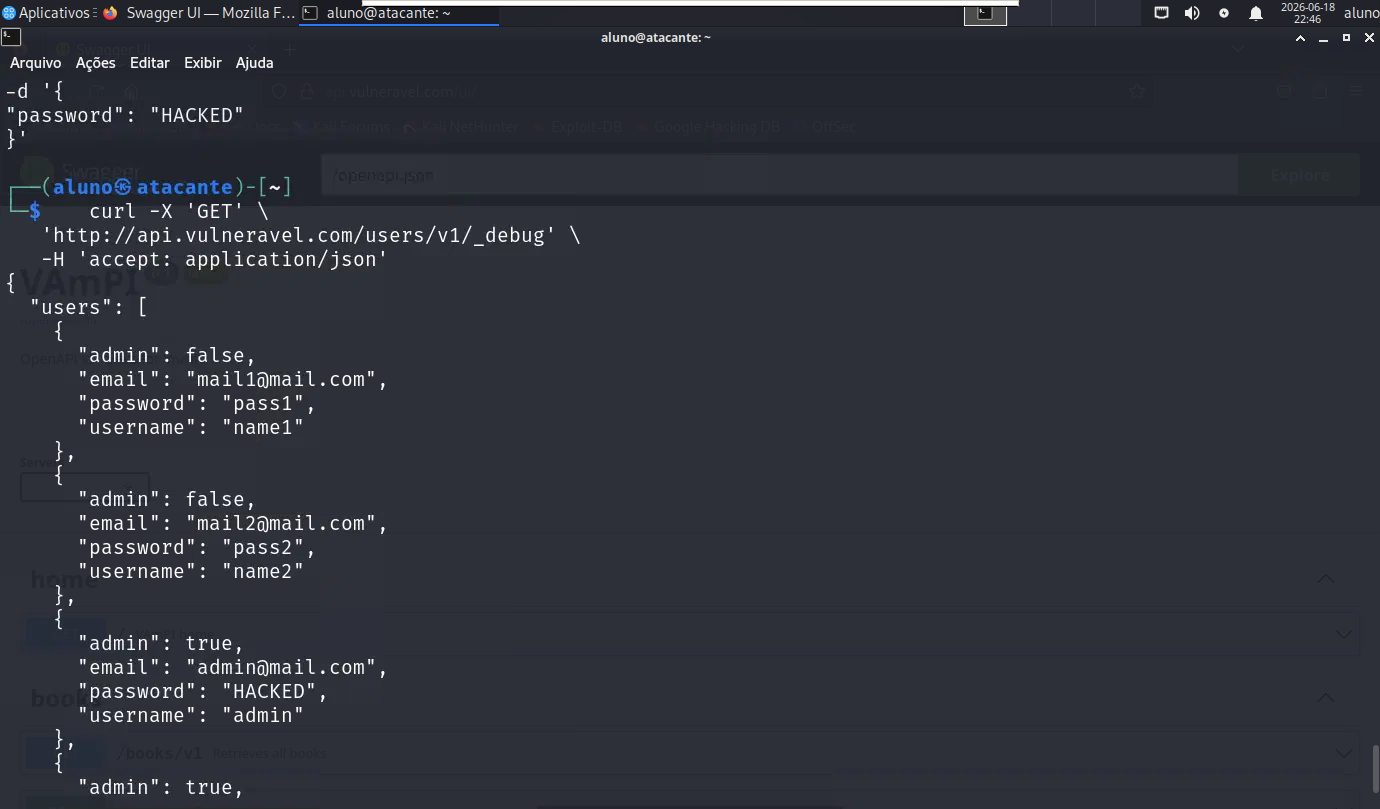
\includegraphics[width=0.95\textwidth]{./fig/unauthorized-password-change.png}
\caption{Alteração não autorizada da senha do usuário administrador de para
\texttt{HACKED}.}
\end{figure}
